% IF YOU ARE USING OVERLEAF, MAKE SURE TO SET THE COMPILER TO XeLatex (Menu in the top left > Settings > Compiler).
% Gemini theme
% See: https://rev.cs.uchicago.edu/k4rtik/gemini-uccs
% A fork of https://github.com/anishathalye/gemini

\documentclass[final]{beamer}

% ====================
% Packages
% ====================

\usepackage[T1]{fontenc}
\usepackage{lmodern}
\usepackage[size=custom,width=120,height=72,scale=1.0]{beamerposter}
\usetheme{gemini}
% \usecolortheme{uchicago}
\usecolortheme{stanford}
\usepackage{graphicx}
\usepackage{booktabs}
\usepackage{tikz}
\usepackage{pgfplots}
\pgfplotsset{compat=1.17}
\usepackage{amsmath}
\usepackage{capt-of}
\graphicspath{{../paper_final/}}

% ====================
% Lengths
% ====================

% If you have N columns, choose \sepwidth and \colwidth such that
% (N+1)*\sepwidth + N*\colwidth = \paperwidth
\newlength{\sepwidth}
\newlength{\colwidth}
\setlength{\sepwidth}{0.025\paperwidth}
\setlength{\colwidth}{0.3\paperwidth}

\newcommand{\separatorcolumn}{\begin{column}{\sepwidth}\end{column}}


\title{FocusFusion: Cross-Attention Fusion of LiDAR and Vision Features for 3D Semantic Segmentation}


\author{Edward Lee \inst{1} \and Ben Saif Moolji \inst{2} \and Umar Padela \inst{3}}


\institute[shortinst]{\inst{1} Computer Science, Stanford \samelineand \inst{2} ICME, Stanford \samelineand \inst{3} Aeronautics and Astronautics, Stanford}

% ====================
% Footer (optional)
% ====================

\footercontent{
  \href{rylanschaeffer.github.io}{rylanschaeffer.github.io} \hfill
  NeurIPS 2021 Workshop: Metacognition in the Age of AI \hfill
  \href{mailto:rylanschaeffer@gmail.com}{rylanschaeffer@gmail.com}}
% (can be left out to remove footer)

% ====================
% Logo (optional)
% ====================

% use this to include logos on the left and/or right side of the header:
% \logoright{\includegraphics[height=7cm]{logos/cs-logo-maroon.png}}
% \logoleft{\includegraphics[height=7cm]{logos/cs-logo-maroon.png}}

% ====================
% Body
% ====================

\begin{document}

% This adds the Logos on the top left and top right
\addtobeamertemplate{headline}{}
{
    \begin{tikzpicture}[remember picture,overlay]
    %   \node [anchor=north west, inner sep=3cm] at ([xshift=0.0cm,yshift=1.0cm]current page.north west)
    %   {\includegraphics[height=5.0cm]{stanford_logos/Stanford-CS.png}}; % uc-logo-white.eps
      \node [anchor=north east, inner sep=3cm] at ([xshift=0.0cm,yshift=2.5cm]current page.north east)
      {
\includegraphics[height=7.0cm]{stanford_logos/Block_S_2_color.png}};
    \end{tikzpicture}
}

\begin{frame}[t]
\begin{columns}[t]
\separatorcolumn

\begin{column}{\colwidth}

  \begin{block}{Introduction}

    Some block contents, followed by a diagram, followed by a dummy paragraph.

    \begin{figure}
      \centering
      \begin{tikzpicture}[scale=6]
        \draw[step=0.25cm,color=gray] (-1,-1) grid (1,1);
        \draw (1,0) -- (0.2,0.2) -- (0,1) -- (-0.2,0.2) -- (-1,0)
          -- (-0.2,-0.2) -- (0,-1) -- (0.2,-0.2) -- cycle;
      \end{tikzpicture}
      \caption{A figure caption.}
    \end{figure}

    Lorem ipsum dolor sit amet, consectetur adipiscing elit. Morbi ultricies
    eget libero ac ullamcorper. Integer et euismod ante. Aenean vestibulum
    lobortis augue, ut lobortis turpis rhoncus sed. Proin feugiat nibh a
    lacinia dignissim. Proin scelerisque, risus eget tempor fermentum, ex
    turpis condimentum urna, quis malesuada sapien arcu eu purus.

  \end{block}

  \begin{block}{Problem Statement}

    Nam vulputate nunc felis, non condimentum lacus porta ultrices. Nullam sed
    sagittis metus. Etiam consectetur gravida urna quis suscipit.

    \begin{itemize}
      \item \textbf{Mauris tempor} risus nulla, sed ornare
      \item \textbf{Libero tincidunt} a duis congue vitae
      \item \textbf{Dui ac pretium} morbi justo neque, ullamcorper
    \end{itemize}

    Eget augue porta, bibendum venenatis tortor.

  \end{block}
  
    \begin{block}{Dataset}
    
    \end{block}

  \begin{alertblock}{A highlighted block}

    This block catches your eye, so \textbf{important stuff} should probably go
    here.

    Curabitur eu libero vehicula, cursus est fringilla, luctus est. Morbi
    consectetur mauris quam, at finibus elit auctor ac. Aliquam erat volutpat.
    Aenean at nisl ut ex ullamcorper eleifend et eu augue. Aenean quis velit
    tristique odio convallis ultrices a ac odio.

    \begin{itemize}
      \item \textbf{Fusce dapibus tellus} vel tellus semper finibus. In
        consequat, nibh sed mattis luctus, augue diam fermentum lectus.
      \item \textbf{In euismod erat metus} non ex. Vestibulum luctus augue in
        mi condimentum, at sollicitudin lorem viverra.
      \item \textbf{Suspendisse vulputate} mauris vel placerat consectetur.
        Mauris semper, purus ac hendrerit molestie, elit mi dignissim odio, in
        suscipit felis sapien vel ex.
    \end{itemize}

    Aenean tincidunt risus eros, at gravida lorem sagittis vel. Vestibulum ante
    ipsum primis in faucibus orci luctus et ultrices posuere cubilia Curae.

  \end{alertblock}

\end{column}

\separatorcolumn

\begin{column}{\colwidth}

  \begin{block}{Methods}

    Vivamus congue volutpat elit non semper. Praesent molestie nec erat ac
    interdum. In quis suscipit erat. \textbf{Phasellus mauris felis, molestie
    ac pharetra quis}, tempus nec ante. Donec finibus ante vel purus mollis
    fermentum. Sed felis mi, pharetra eget nibh a, feugiat eleifend dolor. Nam
    mollis condimentum purus quis sodales. Nullam eu felis eu nulla eleifend
    bibendum nec eu lorem. Vivamus felis velit, volutpat ut facilisis ac,
    commodo in metus.



  \end{block}

  \begin{block}{Experiments \& Analysis}

    \vspace{1ex}
    \begin{columns}[t]
      \begin{column}{0.43\linewidth}
        \normalsize
        \begin{tabular}{lccc}
          \toprule
          \textbf{Method} & \textbf{mIoU} & \textbf{mAcc} & \textbf{fwIoU} \\
          \midrule
          LitePT & 0.606 & 0.808 & \textbf{0.911} \\
          \textbf{FocusFusion} & \textbf{0.810} & \textbf{0.876} & 0.903 \\
          \bottomrule
        \end{tabular}
      \end{column}
      \begin{column}{0.54\linewidth}
        \vspace*{-\abovecaptionskip}
        \captionof{table}{Baseline: LitePT vs.\ FocusFusion. \textbf{+20.4\% mIoU} from fusing visual patch features, which help disambiguate geometry-ambiguous classes (e.g.\ poles vs.\ pedestrians look nearly identical in LiDAR alone).}
      \end{column}
    \end{columns}

    \begin{figure}
      \centering
      \begin{minipage}[b]{0.499\linewidth}
        \centering
        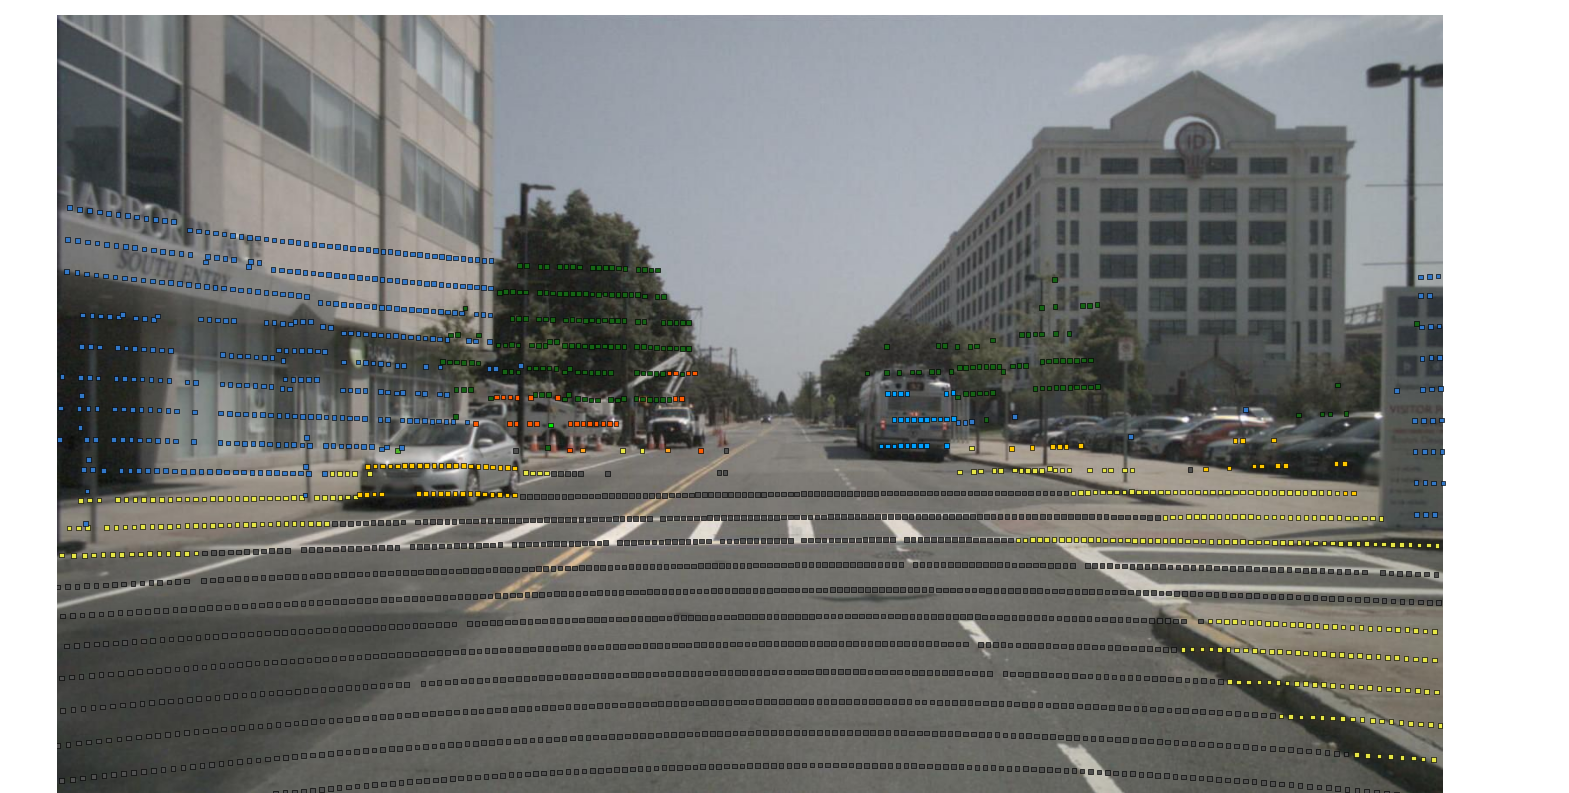
\includegraphics[width=\linewidth]{groundtruth_modal_comp/groundtruth1_cropped.png}
      \end{minipage}%
      \begin{minipage}[b]{0.499\linewidth}
        \centering
        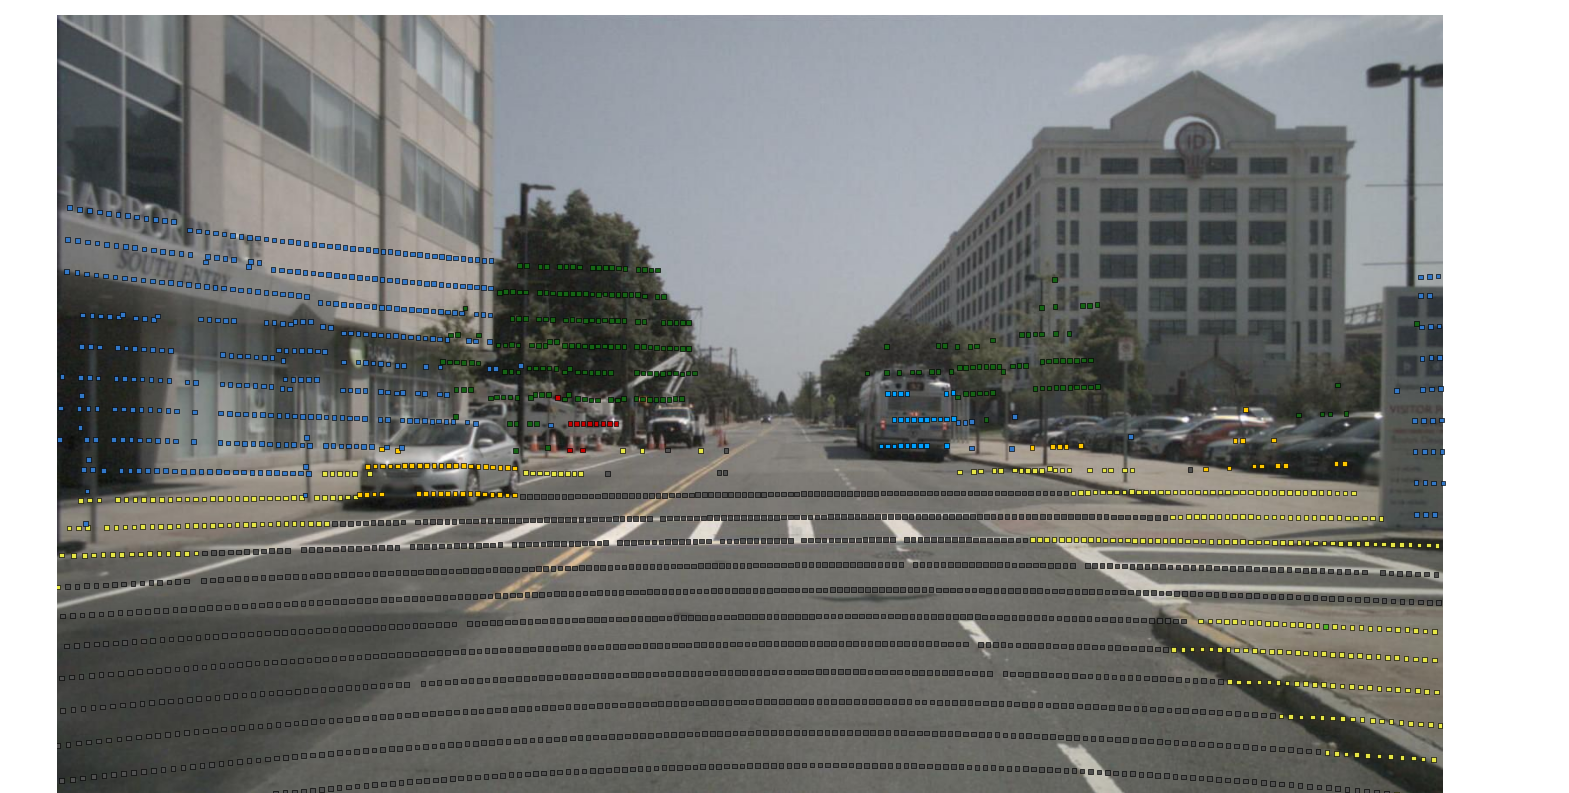
\includegraphics[width=\linewidth]{groundtruth_modal_comp/model1_cropped.png}
      \end{minipage}\\[0.3ex]
      
\includegraphics[width=0.75\linewidth]{groundtruth_modal_comp/legend1.png}
      \caption{Ground Truth (left) vs.\ FocusFusion Prediction (right). LiDAR points projected onto the front camera and colored by semantic class. Road, vegetation, and vehicles are well-segmented; main failures are sidewalk/terrain confusion and missed traffic cones.}
    \end{figure}

    \begin{columns}[t]
      \begin{column}{0.68\linewidth}
        \centering
        \begin{minipage}[b]{0.485\linewidth}
          \centering
          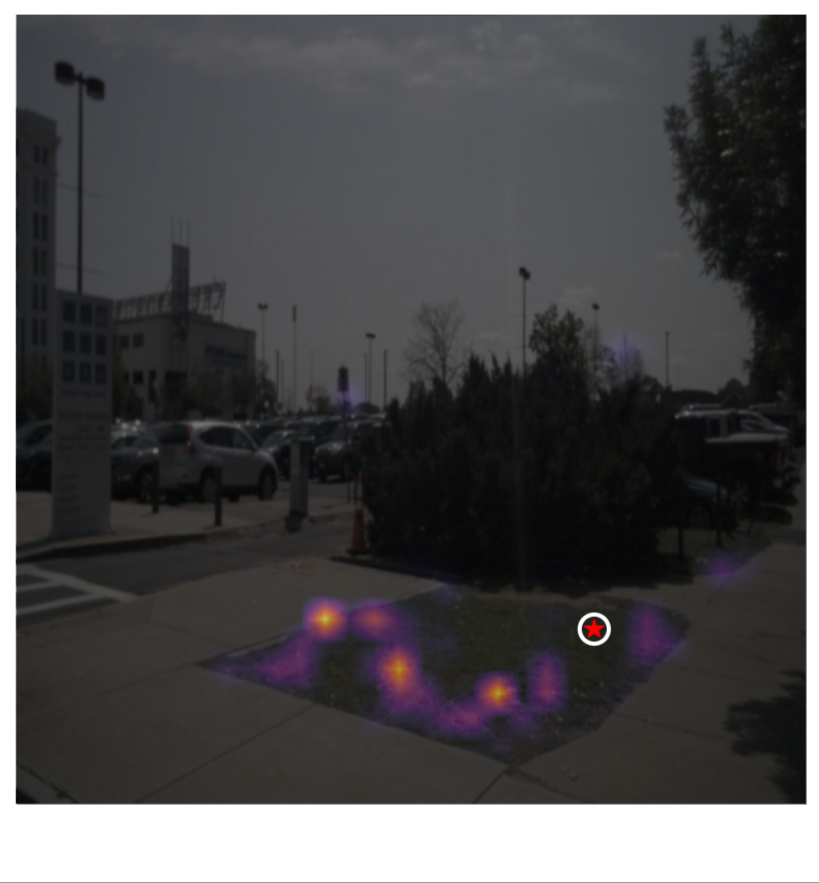
\includegraphics[width=\linewidth]{attention_map_figures/lidar_terrain.png}
        \end{minipage}%
        \hspace{0.03\linewidth}%
        \begin{minipage}[b]{0.485\linewidth}
          \centering
          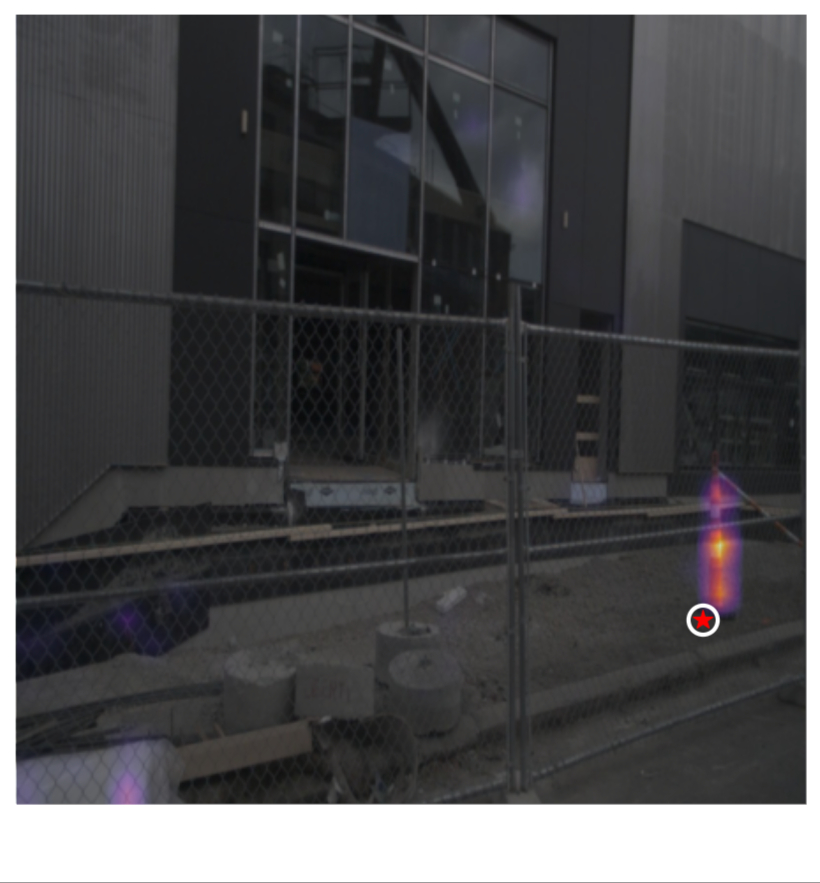
\includegraphics[width=\linewidth]{attention_map_figures/attention_map_traffic_cone.png}
        \end{minipage}
      \end{column}
      \begin{column}{0.28\linewidth}
        \vspace*{-28ex}
        \captionof{figure}{Cross-attention maps: terrain query (left), traffic cone query (right). Warmer colors indicate higher attention weight. Terrain: diffuse attention over grass. Traffic cone: sharp spike on orange patches. Correspondences learned \textbf{without any calibration}.}
      \end{column}
    \end{columns}

  \end{block}

 

\end{column}

\separatorcolumn

\begin{column}{\colwidth}

  \begin{block}{Ablation Studies}

    \begin{columns}[t]
      \begin{column}{0.44\linewidth}
        \normalsize
        \begin{tabular}{lccc}
          \toprule
          Features & mIoU & mAcc & fwIoU \\
          \midrule
          L12 only ($D_v{=}384$) & 0.683 & \textbf{0.798} & \textbf{0.909} \\
          L9+L12 ($D_v{=}768$) & \textbf{0.685} & 0.782 & 0.907 \\
          \bottomrule
        \end{tabular}
      \end{column}
      \begin{column}{0.53\linewidth}
        \vspace*{-\abovecaptionskip}
        \captionof{table}{DINOv2 layer selection. Negligible gain from doubling $D_v$; L12 alone is sufficient at this data scale.}
      \end{column}
    \end{columns}
    \begin{figure}
      \centering
      \begin{minipage}[b]{0.18\linewidth}
        \centering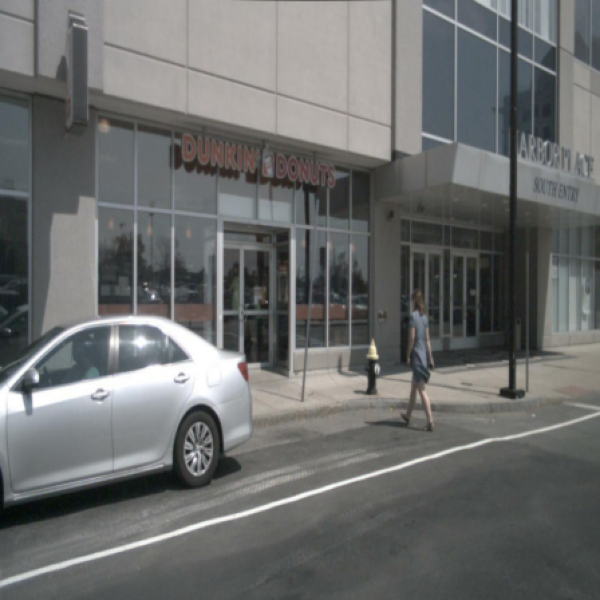
\includegraphics[width=\linewidth]{DINO_PCA/raw_img_DINO_PCA.png}
      \end{minipage}\hfill%
      \begin{minipage}[b]{0.18\linewidth}
        \centering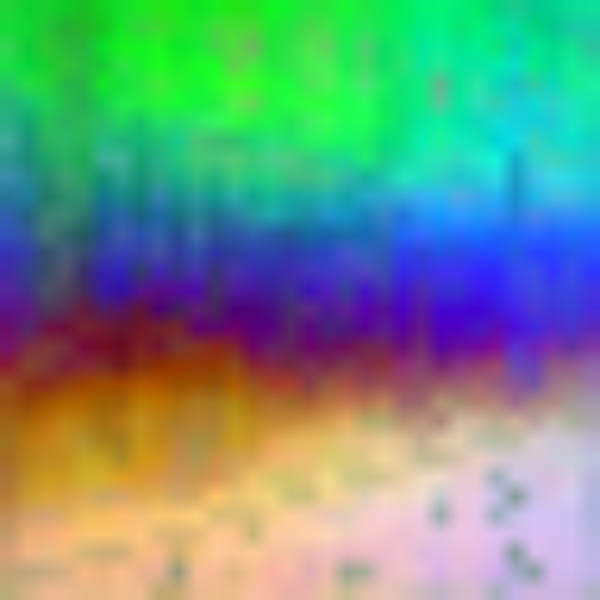
\includegraphics[width=\linewidth]{DINO_PCA/layer9_DINO_PCA.png}
      \end{minipage}\hfill%
      \begin{minipage}[b]{0.18\linewidth}
        \centering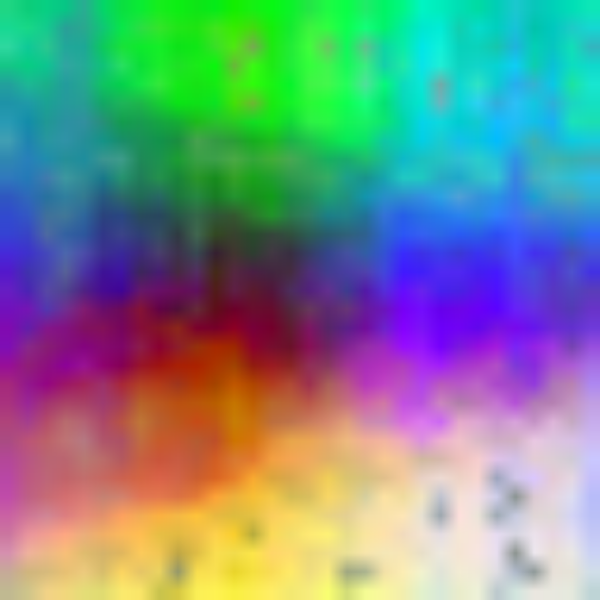
\includegraphics[width=\linewidth]{DINO_PCA/layer10_DINO_PCA.png}
      \end{minipage}\hfill%
      \begin{minipage}[b]{0.18\linewidth}
        \centering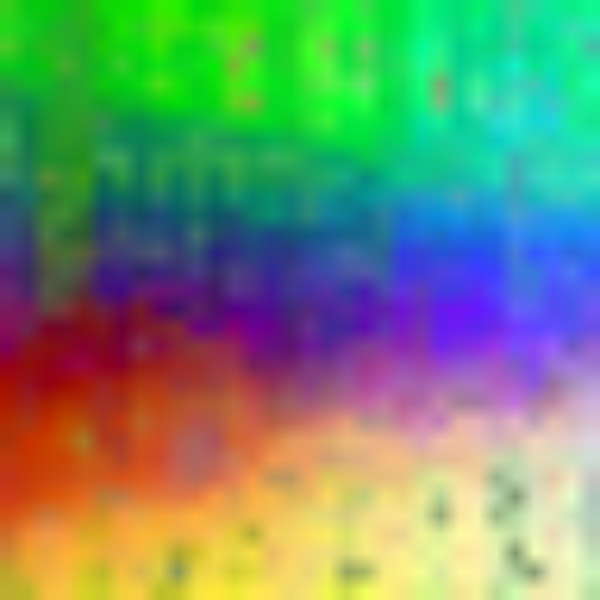
\includegraphics[width=\linewidth]{DINO_PCA/layer11_DINO_PCA.png}
      \end{minipage}\hfill%
      \begin{minipage}[b]{0.18\linewidth}
        \centering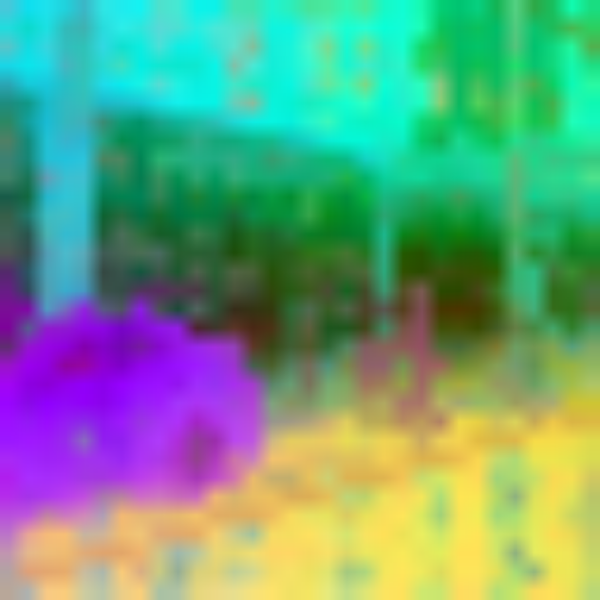
\includegraphics[width=\linewidth]{DINO_PCA/layer12_DINO_PCA.png}
      \end{minipage}
      \caption{PCA of DINOv2 patch embeddings (raw image, L9--L12). Deeper layers resolve increasingly fine object boundaries.}
    \end{figure}

    \vspace{1ex}\noindent
    \begin{minipage}[t]{0.48\linewidth}
      \centering\normalsize
      \begin{tabular}{cccc}
        \toprule
        $\lambda$ & mIoU & mAcc & fwIoU \\
        \midrule
        0    & 0.639 & \textbf{0.809} & 0.903 \\
        \textbf{0.25} & \textbf{0.683} & 0.798 & 0.909 \\
        0.5  & 0.681 & 0.783 & \textbf{0.910} \\
        \bottomrule
      \end{tabular}
      \captionof{table}{Lov\'asz loss weight $\lambda$. $\lambda{=}0.25$ optimal; pure CE biases toward common classes and $\lambda{=}0.5$ over-penalizes, degrading mAcc.}
    \end{minipage}
    \hfill
    \begin{minipage}[t]{0.48\linewidth}
      \centering\normalsize
      \begin{tabular}{cccc}
        \toprule
        $T$ & mIoU & mAcc & fwIoU \\
        \midrule
        \textbf{1} & \textbf{0.810} & \textbf{0.876} & \textbf{0.903} \\
        6 (3\,s) & 0.806 & 0.875 & 0.902 \\
        \bottomrule
      \end{tabular}
      \captionof{table}{Temporal memory bank depth $T$. $T{=}1$ wins at this data scale; longer $K/V$ sequences need more training diversity to supervise.}
    \end{minipage}

  \end{block}

  \begin{block}{Conclusions \& Future Work}

    Class aptent taciti sociosqu ad litora torquent per conubia nostra, per
    inceptos himenaeos. Phasellus libero enim, gravida sed erat sit amet,
    scelerisque congue diam. Fusce dapibus dui ut augue pulvinar iaculis.

    \begin{table}
      \centering
      \begin{tabular}{l r r c}
        \toprule
        \textbf{First column} & \textbf{Second column} & \textbf{Third column} & \textbf{Fourth} \\
        \midrule
        Foo & 13.37 & 384,394 & $\alpha$ \\
        Bar & 2.17 & 1,392 & $\beta$ \\
        Baz & 3.14 & 83,742 & $\delta$ \\
        Qux & 7.59 & 974 & $\gamma$ \\
        \bottomrule
      \end{tabular}
      \caption{A table caption.}
    \end{table}

    Donec quis posuere ligula. Nunc feugiat elit a mi malesuada consequat. Sed
    imperdiet augue ac nibh aliquet tristique. Aenean eu tortor vulputate,
    eleifend lorem in, dictum urna. Proin auctor ante in augue tincidunt
    tempor. Proin pellentesque vulputate odio, ac gravida nulla posuere
    efficitur. Aenean at velit vel dolor blandit molestie. Mauris laoreet
    commodo quam, non luctus nibh ullamcorper in. Class aptent taciti sociosqu
    ad litora torquent per conubia nostra, per inceptos himenaeos.

    Nulla varius finibus volutpat. Mauris molestie lorem tincidunt, iaculis
    libero at, gravida ante. Phasellus at felis eu neque suscipit suscipit.
    Integer ullamcorper, dui nec pretium ornare, urna dolor consequat libero,
    in feugiat elit lorem euismod lacus. Pellentesque sit amet dolor mollis,
    auctor urna non, tempus sem.

  \end{block}

  \begin{block}{References}

    \nocite{*}
    \footnotesize{\bibliographystyle{plain}\bibliography{poster}}

  \end{block}

\end{column}

\separatorcolumn
\end{columns}
\end{frame}

\end{document}
